\documentclass[11pt, oneside]{article}   	% use "amsart" instead of "article" for AMSLaTeX format
\usepackage[margin=1in]{geometry}                		% See geometry.pdf to learn the layout options. There are lots.
\geometry{letterpaper}                   		% ... or a4paper or a5paper or ... 
%\geometry{landscape}                		% Activate for for rotated page geometry
\usepackage[parfill]{parskip}    		% Activate to begin paragraphs with an empty line rather than an indent
\usepackage{graphicx}				% Use pdf, png, jpg, or eps� with pdflatex; use eps in DVI mode
								% TeX will automatically convert eps --> pdf in pdflatex		
\usepackage{amssymb}
\usepackage{mathtools}


\title{ANOVA}
\author{Thomas Elliott}
\date{\today}							% Activate to display a given date or no date

\begin{document}
\maketitle

ANOVA stands for analysis of variance and is one of the basic statistical tests we can use to find relationships between two or more variables. ANOVA compares the group means of a dependent variable where the groups are defined by one or more independent variables. Using ANOVA, we can find out if the group means are statistically significant, but also how much variance in the dependent variable is explained by our independent variables.

\section{Oneway ANOVA}

Oneway ANOVA involves testing the relationship between two and only two variables. Let's consider the example in which income in thousands is our dependent variable and gender, coded male and female, is our independent variable. To do ANOVA, we need to calculate the mean income for each group in our independent variable. 

\begin{table}[h]
\centering
\caption{Group Means}
\label{tab:means}
\begin{tabular}{l c c}
\hline
Group & Mean & N\\
\hline
Male & 49.9 & 95\\
Female & 30.9 & 105\\
\hline
Total & 39.9 & 200\\
\hline
\end{tabular}
\end{table}

\subsection{Sum of Squares}

ANOVA involves calculating three different sums of squares. Each also has an associated degrees of freedom (\(df\)), with N = number of cases and K = number of groups. First, the total sum of squares (TSS) is the sum of the square deviations of each case from the grand or total mean:

\[
\textrm{TSS} = \sum (Y - \bar{Y}_{grand} )^2 
\]
\[ df = N- 1 \]

Second, the within sum of squares (WSS), which is also called the residual sum of squares or the error sum of squares, is the sum of the square deviations of each case from their group mean:

\[
\textrm{WSS} = \sum (Y - \bar{Y}_{group} )^2
\]
\[ df = N - K \]

Third, the between sum of squares (BSS), which is also called the explained sum of squares, the regression sum of squares, or the model sum of squares, is the sum of the square deviations of the group means from the grand mean for each case.

\[
\textrm{BSS} = \sum (\bar{Y}_{group} - \bar{Y}_{grand} )^2
\]
\[ df = K - 1 \]

Table \ref{tab:tss} shows how to calculate TSS by hand with a sample of the data presented in Table \ref{tab:means}. You calculate the deviation of each income from the grand mean by subtracting the grand mean from the individual scores. Then you square the deviation, and then sum the squares. Tables \ref{tab:wss} and \ref{tab:bss} show how to compute WSS and BSS respectively.

\begin{table}[h]
\centering
\caption{Calculating TSS}
\label{tab:tss}
\begin{tabular}{*{6}{c}}
\hline
Case & Gender & Income & Grand Mean & Deviation & Sqr Dev\\ \hline
1 & Male & 59.3 & 39.9 & 19.4 & 376.36 \\
2 & Male & 46.5 & 39.9 & 6.6 & 43.56\\
3 & Male & 49.7 & 39.9 & 9.8 & 96.04 \\
4 & Male & 45.7 & 39.9 & 5.8 & 33.64 \\
5 & Male & 46.9 & 39.9 & 7 & 49 \\
6 & Female & 32.2 & 39.9 & -7.7 & 59.29\\ 
7 & Female & 36.5 & 39.9 & -3.4 & 11.56 \\
8 & Female & 28.9 & 39.9 & -11 & 121 \\
9 & Female & 49.5 & 39.9 & 9.6 & 92.16 \\
10& Female & 33.1 & 39.9 & -6.8 & 46.24 \\
\hline
 & & & & TSS: & 928.85\\
\hline
\end{tabular}
\end{table}

\begin{table}[h]
\centering
\caption{Calculating WSS}
\label{tab:wss}
\begin{tabular}{*{6}{c}}
\hline
Case & Gender & Income & Group Mean & Deviation & Sqr Dev\\ \hline
1 & Male & 59.3 & 49.9 & 9.4 & 88.36 \\
2 & Male & 46.5 & 49.9 & -3.6 & 11.56\\
3 & Male & 49.7 & 49.9 & -0.2 & 0.04 \\
4 & Male & 45.7 & 49.9 & -4.2 & 17.64 \\
5 & Male & 46.9 & 49.9 & -3 & 9 \\
6 & Female & 32.2 & 30.9 & 1.3 & 1.69\\ 
7 & Female & 36.5 & 30.9 & 5.6 & 31.36 \\
8 & Female & 28.9 & 30.9 & -2 & 4 \\
9 & Female & 49.5 & 30.9 & 18.6 & 345.96 \\
10& Female & 33.1 & 30.9 & 2.2 & 4.84 \\
\hline
& & & & & 514.45\\
\hline
\end{tabular}
\end{table}

\begin{table}[h]
\centering
\caption{Calculating BSS}
\label{tab:bss}
\begin{tabular}{*{6}{c}}
\hline
Case & Gender & Group Mean & Grand Mean & Deviation & Sqr Dev\\ \hline
1 & Male & 49.9 & 39.9 & 10 & 100 \\
2 & Male & 49.9 & 39.9 & 10 & 100\\
3 & Male & 49.9 & 39.9 & 10 & 100 \\
4 & Male & 49.9 & 39.9 & 10 & 100 \\
5 & Male & 49.9 & 39.9 & 10 & 100 \\
6 & Female & 30.9 & 39.9 & -9 & 81\\ 
7 & Female & 30.9 & 39.9 & -9 & 81 \\
8 & Female & 30.9 & 39.9 & -9 & 81 \\
9 & Female & 30.9 & 39.9 & -9 & 81 \\
10& Female & 30.9 & 39.9 & -9 & 81 \\
\hline
& & & & & 905\\
\hline
\end{tabular}
\end{table}

Since these tables only use 10 of the 200 cases, these are not the final sums of squares for our ANOVA. The sum of squares for the full sample is in Table \ref{tab:ss}. 

\begin{table}[h]
\centering
\caption{Sum of Squares}
\label{tab:ss}
\begin{tabular}{l *{2}{c}}
\hline
& Sum of Squares & Degrees of Freedom\\
\hline
Between & 17929.5 & 1\\
Within & 20448.3 & 198\\
\hline
Total & 38377.8 & 199\\
\hline
\end{tabular}
\end{table}

\subsection{F-Test}

We use these sum of squares to calculate F, our statistic for whether there is a significant difference in group means. F is a ratio of the between mean squares to the within mean squares. Mean squares are themselves a ratio, with the sum of squares divided by the degrees of freedom. 


\[ F = \cfrac{\dfrac{BSS}{K-1}}{\dfrac{WSS}{N-K}} = \frac{BMS}{WMS} \]

\[ F = \cfrac{\dfrac{17929.5}{1}}{\dfrac{20448.3}{198}} = 173.61 \]


This gives us the F-statistic, but now we need figure out if this is large enough to be significant. We do that by looking up critical values of F for a given alpha. There are different tables for different levels of alpha, usually 0.10, 0.05, and 0.01. The table in Figure \ref{fig:ftable} contains the critical values of F for \(\alpha = 0.05\). Along the columns are values of degrees of freedom for the numerator, or the between sum of squares. Along the rows are values of degrees of freedom for the denominator, or the within sum of squares. Our BSS df is 1, and our WSS df is 198, so we look down the column for 1 df and look for the row for 198 df. In this table, the largest df the rows go to is 120, and then it has a row for infinity, for degrees of freedom that are very large. We can use this row. So our critical value if 3.84. If our F-statistic is larger than the critical value, then we have a significant difference in group means (we are able to reject our null hypothesis that the group means are equal). 


\begin{figure}[h]
\centering
\caption{Critical Values of F for \(\alpha\) = 0.05}
\label{fig:ftable}
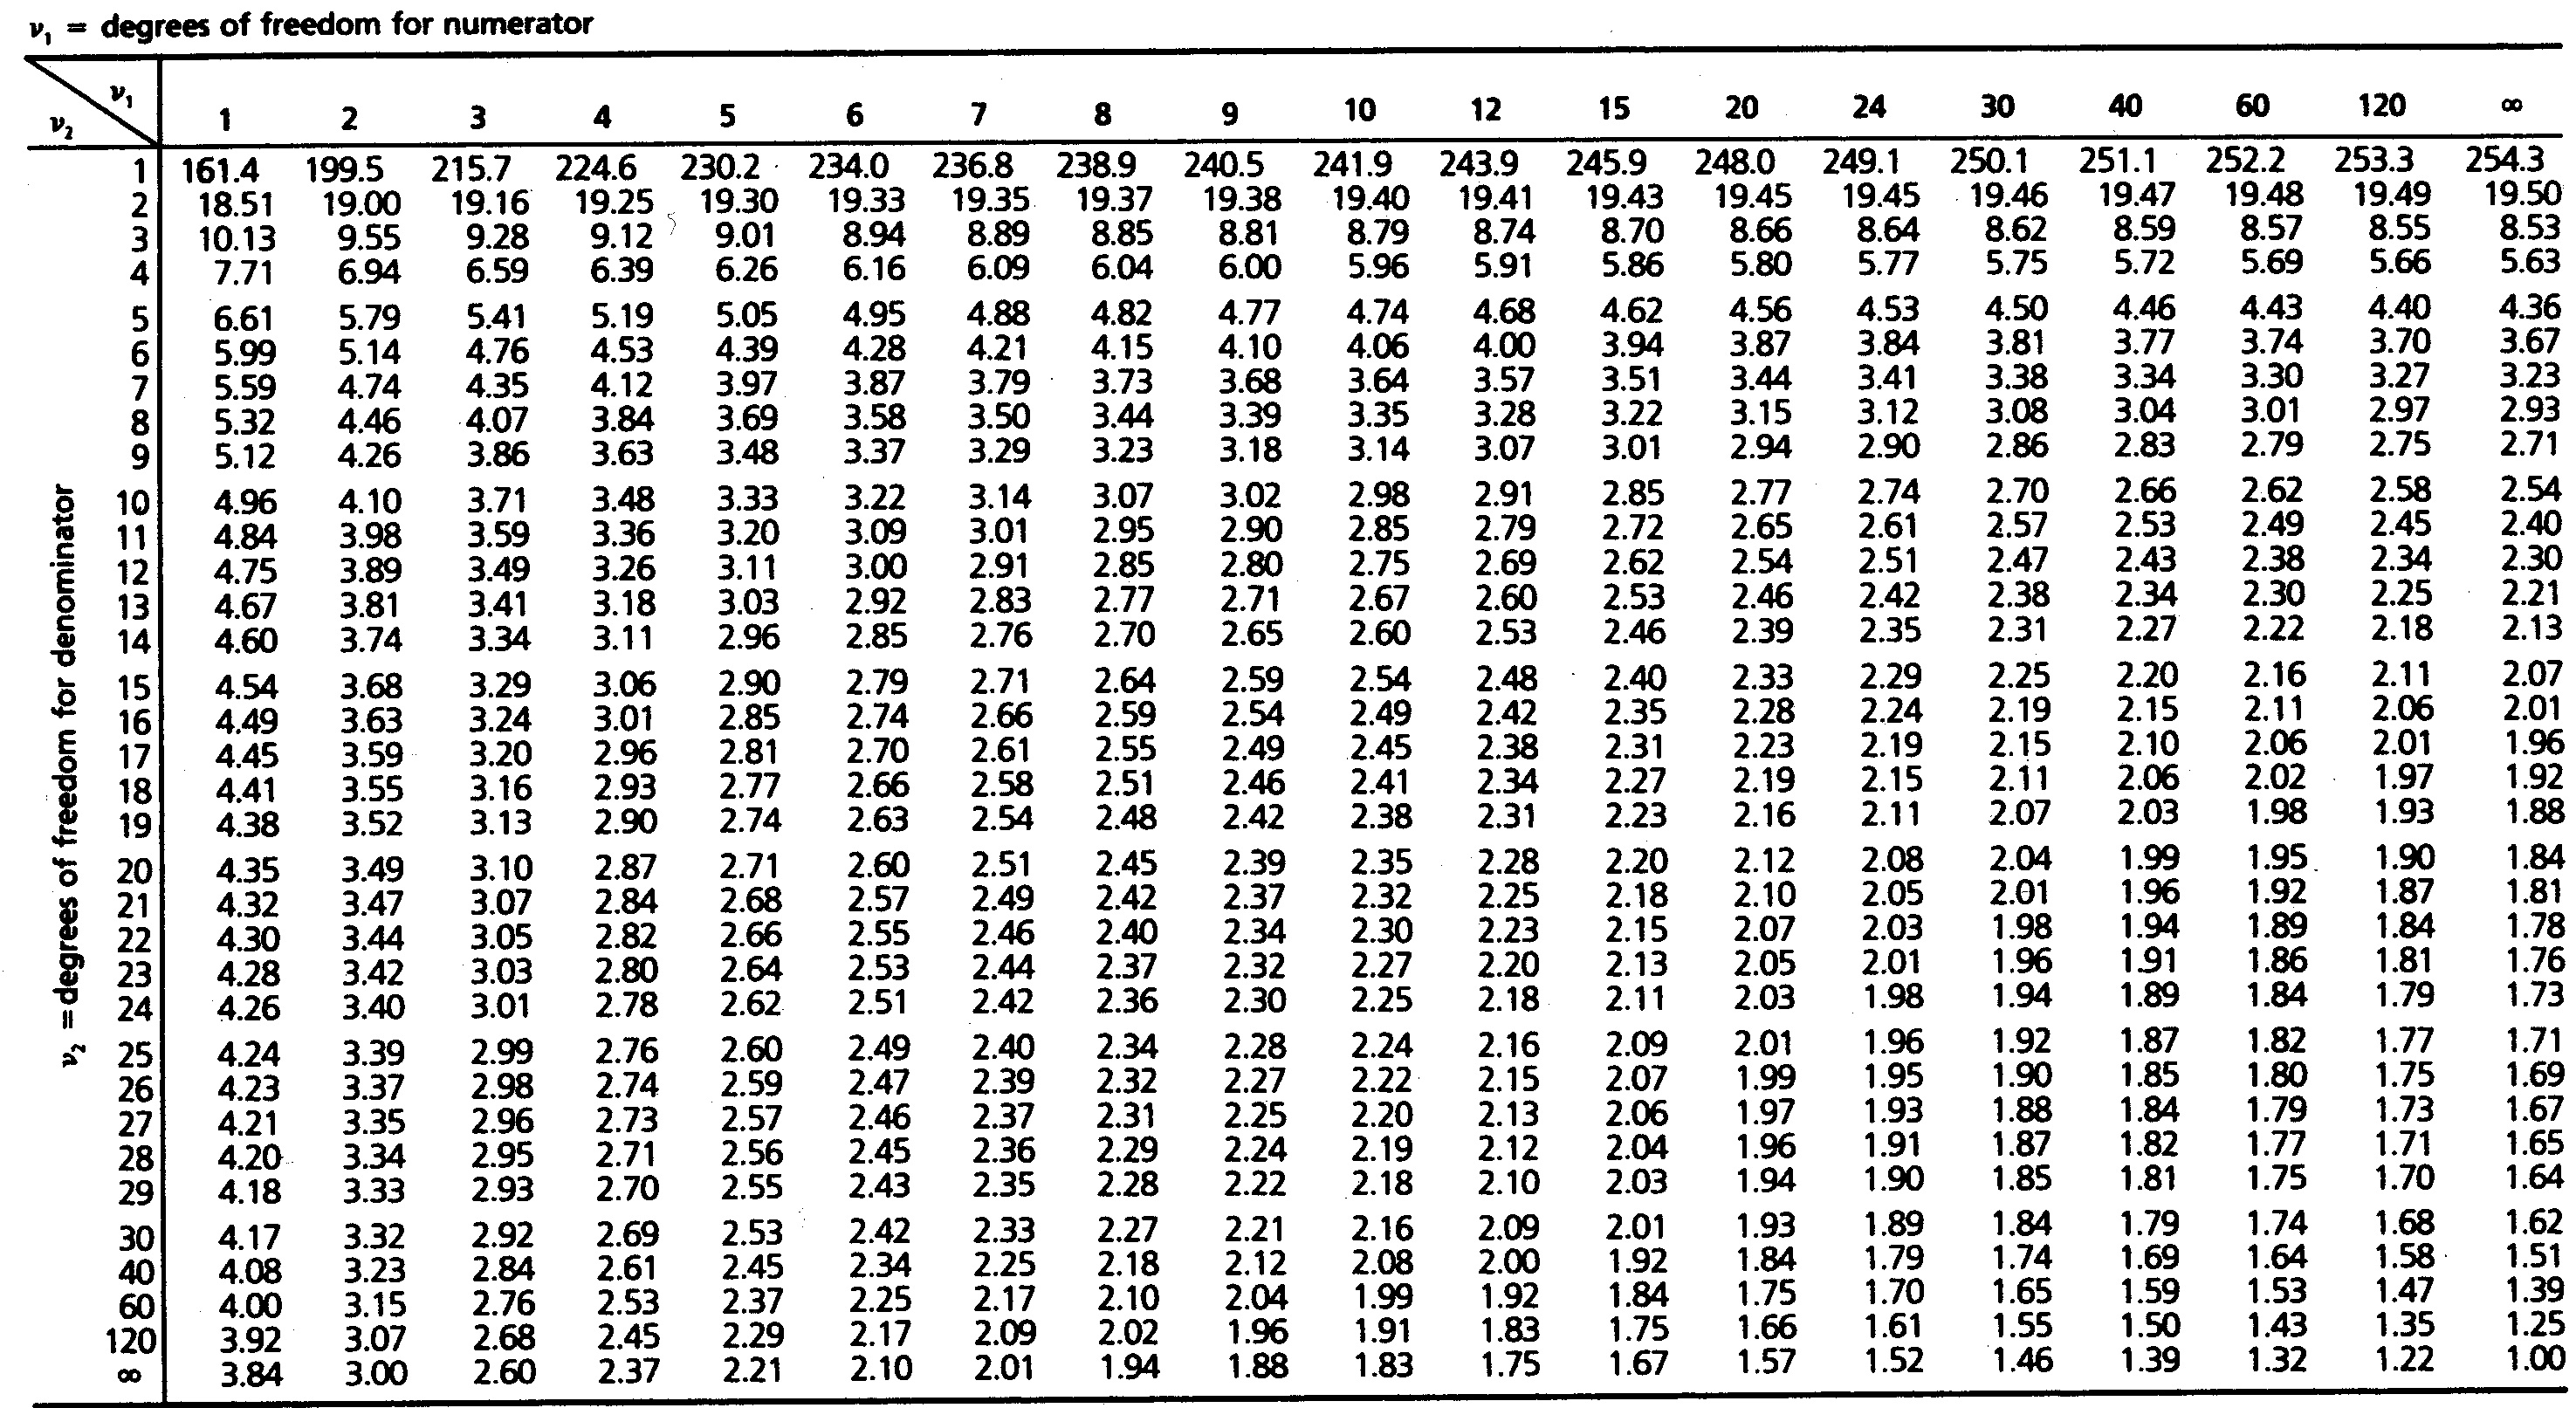
\includegraphics[width=\textwidth]{ftable_crop}
\end{figure}

\subsection{Oneway ANOVA in Stata}

To perform oneway ANOVAs in Stata, use the \texttt{anova} command followed by your dependent variable then your independent variable:

\begin{verbatim}
. anova income gender

                           Number of obs =     200     R-squared     =  0.4672
                           Root MSE      = 10.1624     Adj R-squared =  0.4645

                  Source |  Partial SS    df       MS           F     Prob > F
              -----------+----------------------------------------------------
                   Model |  17929.5346     1  17929.5346     173.61     0.0000
                         |
                  gender |  17929.5346     1  17929.5346     173.61     0.0000
                         |
                Residual |  20448.2833   198  103.274158   
              -----------+----------------------------------------------------
                   Total |  38377.8179   199  192.853356   

\end{verbatim}

As you can see, Stata gives us the model (between), residual (within), and total sums of squares, the degrees of freedom, the mean sums of squares, and the F statistic. 

\section{ANOVA with two or more independent variables}

We are not restricted to only two variables with ANOVA. We can investigate whether there is a relationship among three or more variables. In other words, we can see if our dependent variable varies according to values of two or more categorical independent variables. When we do this, we are investigating whether variable A has an effect on our dependent variable in the presence of, or controlling for, variable B. Sometimes this is referred to as factorial ANOVA.

Extending our example from before, let's say we add an education variable. It has three categories for arbitrarily low, medium, and high levels of education. The income means and frequencies of each group defined by gender and education are in Table \ref{tab:gendereducmeans}.

\begin{table}[h]
\centering
\caption{Means and Frequencies of Income}
\label{tab:gendereducmeans}
\begin{tabular}{l | c c c | r}
\hline
Gender & Low & Medium & High & Total\\
\hline \hline
Female & 21.24 & 36.23 & 53.14 & 30.90\\
& 43 & 57 & 5 & 105\\
\hline
Male & 25.53 & 41.18 & 57.33 & 49.86\\
& 1 & 42 & 52 & 95\\
\hline
Total & 21.34 & 38.33 & 56.96 & 39.90\\
& 44 & 99 & 57 & 200\\
\hline
\end{tabular}
\end{table}

It looks like there is a relationship between education and income, as well as between sex and income. Often, we'll want to test not only if a relationship exists between the two independent variables and the dependent variable, but if the effect on one variable depends on the value of the other variable. In our example, we could imagine that the effect of education on income might be different depending on whether the case is a man or a woman. In regression analysis, we would say the slopes of income on education differ for men and women. When this happens, we call it an interaction effect. Two independent variables are interacting with one another to produce the dependent variable. We often include interaction terms in factorial ANOVA. 

To perform a factorial ANOVA in Stata, we use the \texttt{anova} command:

\begin{verbatim}
. anova income gender educ gender#educ

                           Number of obs =     200     R-squared     =  0.8518
                           Root MSE      = 5.41373     Adj R-squared =  0.8480

                  Source |  Partial SS    df       MS           F     Prob > F
            -------------+----------------------------------------------------
                   Model |  32691.9761     5  6538.39521     223.09     0.0000
                         |
                  gender |  140.544649     1  140.544649       4.80     0.0297
                   educ  |  5411.68372     2  2705.84186      92.32     0.0000
            gender#educ  |  2.50078462     2  1.25039231       0.04     0.9582
                         |
                Residual |  5685.84179   194  29.3084628   
            -------------+----------------------------------------------------
                   Total |  38377.8179   199  192.853356   
\end{verbatim}

Like in \texttt{oneway} we type the dependent variable immediately after the command, then a list of our independent variables. Notice what we had to do for our interaction term. In Stata, we specify an interaction term with the pound sign (\#). We could have also typed the command:

 \texttt{anova income gender\#\#educ}
 
This would have produced the same results. Typing two pound signs in a row tells Stata include all possible combinations of variables, making it easier to specify three-way interactions (interactions between three, or more, variables). For more information about how Stata works with factorial variables, you can type \texttt{help fvvarlist}. 

If we look back at our results, we'll find several F-tests. Let's go from bottom to top. The first F-test is for the interaction term. Here the interaction term is testing whether the effect of education on income depends on the value of gender (or whether the effect of gender on income depends on the value of education, both are correct). If we think about the two by two table of means (Table \ref{tab:gendereducmeans}), the difference in mean income between men and women is different for each value of education. According to our F-test, this is not the case. We have an incredibly small F statistic. So the effect of education on income is the same for men and women (or the effect of gender on income is the same for all values of education). 

The next F-test is for the education term alone. This tests whether the mean income differs among values of education, controlling for gender. We can see from the F-test that this is the case - our F statistic is very large, indicating that the different groups defined by education have different mean incomes. Similarly, the F-test for gender tests whether men and women have different incomes, controlling  for education. This F-test is a little less clear. Our F statistic may be significant depending on the value of \(\alpha\) we choose. Finally, we have the F-test for the overall model. This tests whether the three terms taken overall have significant differences in their groups means. Or we can think about it as using gender, education, and an interaction term is better at predicting income than the grand mean of income by itself.

\subsection{Incremental F-test}

What's nice about Stata is that it does a lot of work for us. For example, each of the F-tests for individual terms in the output above are incremental F-tests. Incremental F-tests test the significance of individual terms, or groups of terms, in a model by comparing that model (called the full model) to a model missing the term or terms you want to test the significance of (this smaller model is called the nested model). Normally, it would be pretty tedious for us to calculate those by hand. To see how it works, though, let's calculate one by hand. We have a full, saturated interaction model above. Let's calculate the incremental F-test for the interaction term. We'll need the additive model to do this. Remember, the additive model is model with no interactions.
\newpage
\begin{verbatim}
. anova income gender educ

                           Number of obs =     200     R-squared     =  0.8518
                           Root MSE      = 5.38722     Adj R-squared =  0.8495

                  Source |  Partial SS    df       MS           F     Prob > F
              -----------+----------------------------------------------------
                   Model |  32689.4753     3  10896.4918     375.45     0.0000
                         |
                  gender |  688.562334     1  688.562334      23.73     0.0000
                    educ |  14759.9407     2  7379.97035     254.29     0.0000
                         |
                Residual |  5688.34257   196   29.022156   
              -----------+----------------------------------------------------
                   Total |  38377.8179   199  192.853356   
\end{verbatim}

So we have our interaction model with Model SS = 32691.98 and df = 5, and we have our additive model with Model SS = 32689.48 and df = 3. The equation for the incremental F-test is:

\[
F = \cfrac{\cfrac{\text{Reg SS, full} - \text{Reg SS, nested}}{df, \text{full} - df, \text{nested}}}{\cfrac{\text{Res SS, full}}{df, \text{full}}}
\]

Where the full model is the model with the interaction terms and the nested model is the additive model. All terms in the nested model should appear in the full model. So if we plug in our values:

\begin{align*}
F &= \cfrac{\cfrac{32691.98 - 32689.48}{5-3}}{\cfrac{5685.84}{194}}\\
	&= \cfrac{\cfrac{2.5}{2}}{29.31}\\
	&= 0.0426
\end{align*}

Which is the same F statistic Stata gave us for the interaction term. When we do an incremental F-test, we are testing the significance of the term(s) we left out of the nested model. Here, we left out the interaction term in the nested model, so that is the F-test we calculated.



\end{document}  